
\newpage
\section{Inherently Interpretable Machine Learning Models}\label{sec:3}

Some models are easy to understand because they're simple, like Linear Regression. With these models, it's straightforward to see how they make predictions.
Then there are models where interpretability is built right into their design, like ProtoPNet. This means that even though they might be more complex, they're designed in a way that makes them easier to interpret.

\subsection{Linear Regression}

\begin{table}[H]
  \centering
  \begin{tabular}{|p{0.17\linewidth}|p{0.77\linewidth}|}
    \hline
    Form of \newline explanation & 
    Internal model parameters \\
    
    \hline
    Interpretation & 
    An increase or change of feature  $x_k$  by one unit increases the prediction for $y$ by $\beta_k$  units when all other feature values remain fixed. \\
    \hline
    Advantages &
    \begin{itemize}[nosep, left=0em]
        \item transparent 
        \item solid statistical history
        \item extensions: e.g. GLM, GAM (less interpretable)
    \end{itemize} \\
    
    \hline
    Disadvantages &
    \begin{itemize}[nosep, left=0em]
        \item can only represent linear relationships 
        \item not suitable if features correlations to strong
        \item interactions must be added manually
    \end{itemize} \\
    
    \hline
    Properties & 
    intrinsic, model-specific, global  \\
    
    \hline
  \end{tabular}
  \caption{Overview XAI - Linear Regression.}
  \label{tab:XAILinReg}
\end{table}

Linear Regression models have a simple structure and often offer a clear and understandable explanation of how the input variables influence the output. In certain scenarios, they can even outperform more complex nonlinear models for prediction tasks.
The Linear Regression model is mathematically represented as follows:
\begin{equation}
    f(X) = \beta_0 + \sum_{j=1}^p X_j\beta_j
\end{equation}
 where $X^T=(X_1,\dots,X_p)$ denotes the input vector.
One of the most commonly used techniques for estimating the parameters $\beta_i$ is called \textit{least squares}. In this method, the objective is to minimize the sum of the squared differences between observed and predicted values:
\begin{equation}
    \min_{\beta} \sum_{t_i}^N \lr{y_i-\beta_0-\sum_{j=1}^p x_j\beta_j}^2
    \label{eq:ls_lr}
\end{equation}
where $(x_1,y_1)\dots(x_N,y_N)$ represent the training data pairs.\cite{hastie2009elements}

Because the combination of features is linear, their effects are additive, allowing for easy separation. An increase of one unit in a feature results in a change in the estimated outcome by the weight assigned to that feature. \\
Figure \ref{fig:LRW} presents a visual representation of interpretability using data from a diabetes dataset\cite{diabetes_dataset}:

\begin{figure}[H]
    \centering
    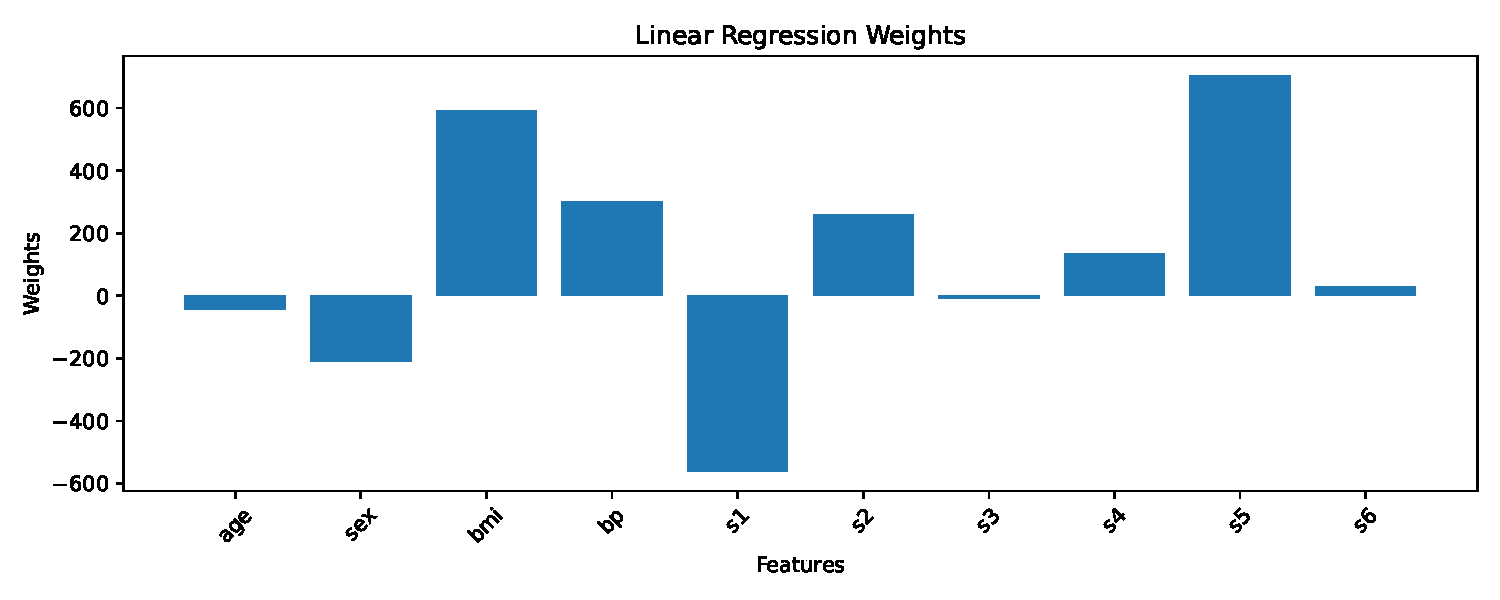
\includegraphics[width=1\linewidth]{pics/Linear_Regression_Weights.pdf}
    \caption[Weights of LR model.]{Weights obtained from a Linear Regression model trained on a diabetes dataset. $bp$ means blood pressure, while $s_1, \dots, s_6$ represent various laboratory values.}
    \label{fig:LRW}
\end{figure}

We observe that the variables $s_5$, $s_1$, and $bmi$ significantly influence the outcome of the model.

However, when dealing with a larger number of features, such as thousands, interpreting the model becomes more challenging. To address this, techniques like variable subset selection or shrinkage methods are used to exclude features with minimal impact on the model's output. \\
A commonly used shrinkage method is the Lasso Regression. This approach introduces a regularization term into the Linear Regression equation \ref{eq:ls_lr} to penalize the coefficients of less influential features:
\begin{equation}
    \min_{\beta} \sum_{t_i}^N \lr{y_i-\beta_0-\sum_{j=1}^p x_j\beta_j}^2 + \lambda \sum_{j=1}^p |\beta_j|.
\end{equation}
Here, $\lambda > 0$ represents the regularization parameter.\cite{hastie2009elements}

Figure \ref{fig:lasso_fit} shows a trace plot of coefficients fit by Lasso Regression, where the regularization parameter $\lambda$ varies within the range of $10^{-4}$ to $10^1$, applied to the diabetes dataset and demonstrates the relationship between $\lambda$ and the coefficients, as well as the resulting mean squared error (MSE):
\begin{figure}[H]
    \centering
    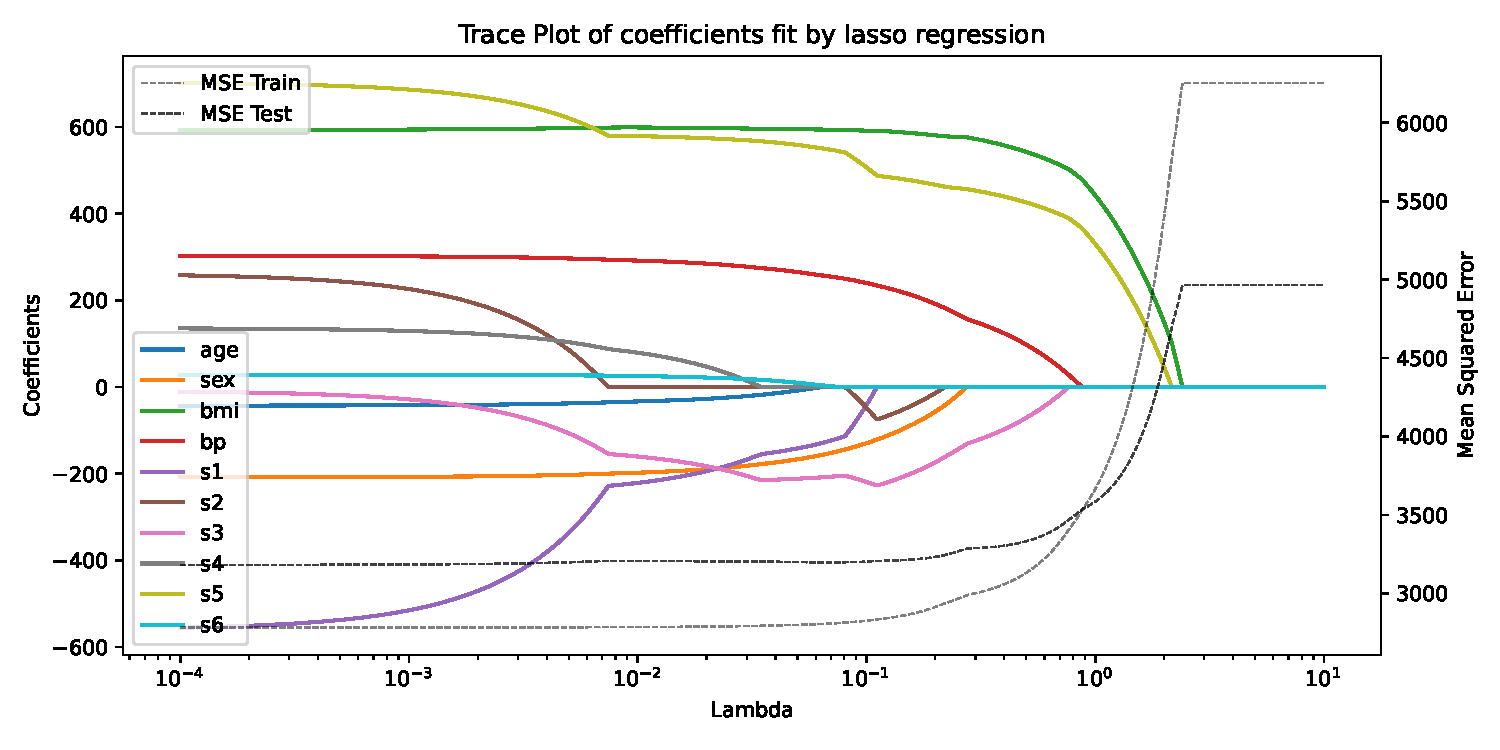
\includegraphics[width=1\linewidth]{pics/Trace_Plot_of_Lasso_Fit.pdf}
    \caption{Trace Plot of coefficients fit by lasso regression.}
    \label{fig:lasso_fit}
\end{figure}

When we observe a value of $\lambda$ slightly greater than $10^{-1}$, we notice that the MSE on the test dataset stopped decreasing. At this point, the model employs only six features, making it simpler to interpret.\\
It's noteworthy that $s_1$ is not among these six features, despite its significant influence on the model output without the regularization term, as displayed in Figure \ref{fig:LRW} (or at $\lambda=10^{-4}$ in Figure \ref{fig:lasso_fit}). This observation encourages the consideration of the limitations inherent in Linear Regression.

Linear Regression is limited in its ability to represent complex relationships as it can only model linear relationships. Nonlinear interactions between variables need to be explicitly defined and provided to the model as input features. \\
Additionally, Linear Regression encounters challenges with correlated features. In cases where features are highly correlated, the increase of one feature by one unit might not accurately correspond to a proportional increase in the prediction for the output by its associated weight, as the model assumes all other feature values remain constant. This can lead to unintuitive weights in the model.\cite{molnar2022}

\subsection{ProtoPNet - \textit{This} Looks Like \textit{That}}\label{sec:ProtoPNet}

\begin{table}[H]
  \centering
  \begin{tabular}{|p{0.17\textwidth}|p{0.77\textwidth}|}
    \hline
    Form of \newline explanation & Points from dataset distribution.
    \\
    
    \hline
    Interpretation & Learned prototypical parts are compared to points from the training dataset.
     \\
 
    \hline
    Advantages &
    \begin{itemize}[nosep, left=0em]
        \item can achieve comparable accuracy with its analogous non-interpretable counterpart
        \item provides a level of interpretability that is absent in other interpretable deep models    
    \end{itemize} \\
    
    \hline
    Disadvantages &
    \begin{itemize}[nosep, left=0em]
        \item (minimal) trade-off in accuracy to best-performing deep models
    \end{itemize} \\
    
    \hline
    Properties & intrinsic, model-specific, local
      \\
    
    \hline
  \end{tabular}
  \caption[Overview XAI - ProtoPNet]{Overview XAI - ProtoPNet.\cite{NEURIPS2019_adf7ee2d}}
  \label{tab:XAIProtoPNet}
\end{table}

In this study \cite{NEURIPS2019_adf7ee2d}, the authors have established a form of interpretability in image processing, which aligns with how humans naturally explain their reasoning in classification tasks.
They introduce a model called the \textit{prototypical part network} (ProtoPNet). The architecture of the network is shown in the following figure:

\begin{figure}[H]
    \centering
    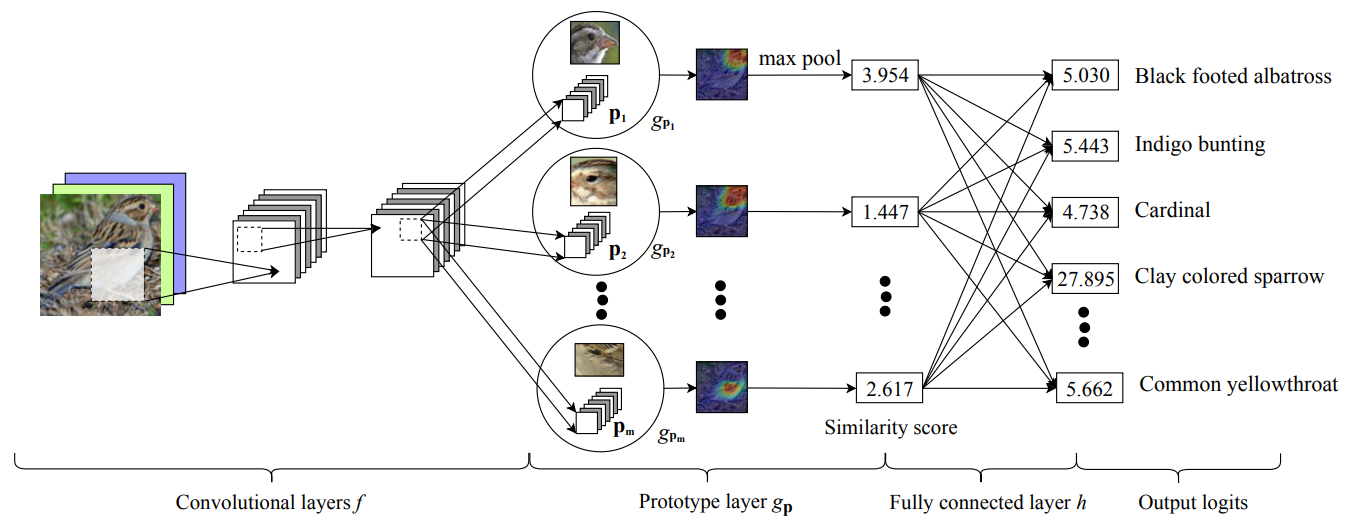
\includegraphics[width=0.9\linewidth]{pics/ProtoPNet_architecture.png}
    \caption[ProtoPNet Architecture.]{ProtoPNet Architecture.\cite{NEURIPS2019_adf7ee2d}}
\end{figure}

This network is designed to break down training images into prototypical parts that represent common identifiable prototypes, such as the head, beak, or wings, which are characteristics of a specific class, like the clay-colored sparrow. Figure \ref{fig:sparrow} shows a demonstration:

\begin{figure}[H]
    \centering
    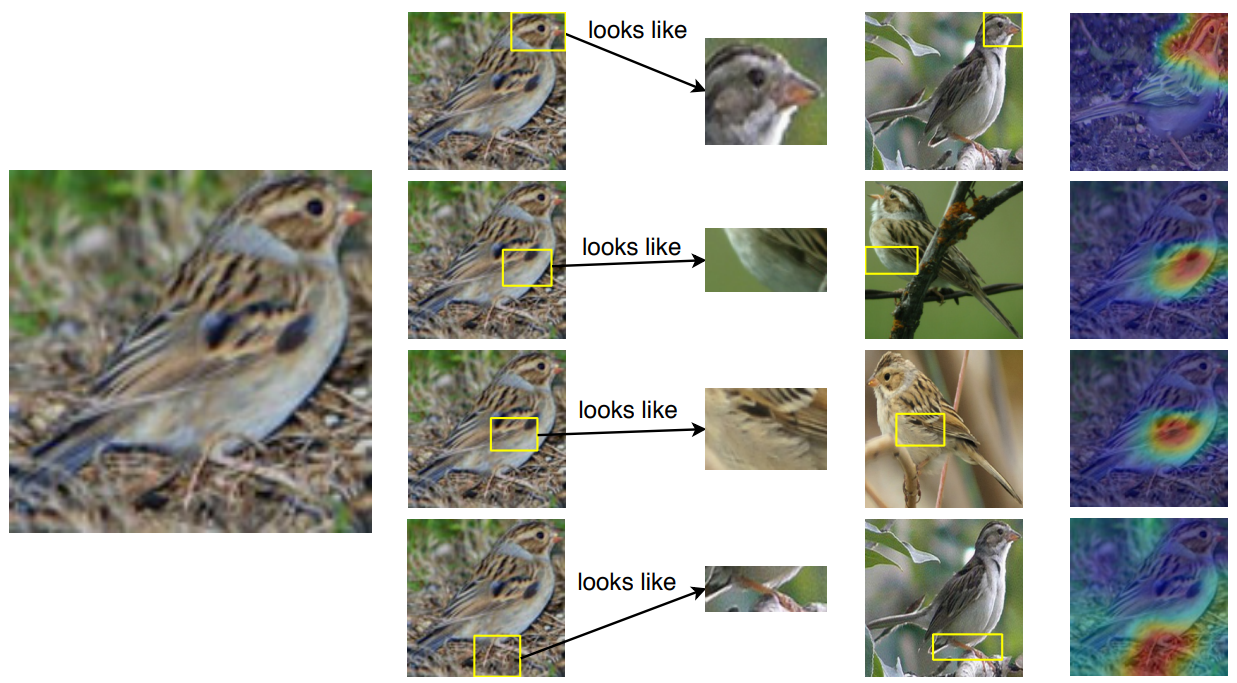
\includegraphics[width=0.7\linewidth]{pics/thisthat.png}
    \caption[Learned prototypical parts of a clay colored sparrow.]{Image of a clay colored sparrow and how parts of it look like some learned prototypical parts of a clay colored sparrow used to classify the bird’s species.\cite{NEURIPS2019_adf7ee2d}}
    \label{fig:sparrow}
\end{figure}

The model then calculates a weighted sum of the similarity between different parts of an input image and the learned prototypes for each class. 

The experiments demonstrate that ProtoPNet can achieve similar accuracy to its comparable non-interpretable counterpart without the Prototype layer. Additionally, ProtoPNet offers a level of interpretability that is lacking in other interpretable deep models.
